% !TEX root = main.tex
\section{Contextual linear Gaussian bandits: baselines}
\label{asec:linearGaussian_baselines}

We show in Figure~\ref{fig:linear_gaussian_mixtures_baselines} the mean cumulative regret (and its standard deviation as the shaded region) of all the studied multi-armed bandit algorithms for diverse contextual linear Gaussian bandit parameterizations ---per-algorithm cumulative reward results are shown in Table~\ref{tab:sparse_linear_showdown_baselines_reward}.

% Linear and Sparse Gaussian reward figure
\begin{table*}[!h]
	\caption{Cumulative reward (mean and variance) at $t=1500$ for $R=500$ realizations of contextual linear Gaussian MABs.}
	\label{tab:sparse_linear_showdown_baselines_reward}
	\vspace*{-2ex}
	\begin{center}
		\resizebox{\textwidth}{!}{
		\begin{tabular}{|c|c|c|}
			\hline
			Algorithm 	\cellcolor[gray]{0.6} & Final cumulative reward (linear) \cellcolor[gray]{0.6} & Final cumulative reward (sparse linear) \cellcolor[gray]{0.6} \\ \hline
			Optimal 	 	 		& 2064.985 $\pm$ 4502.593 & 1960.926 $\pm$ 6363.005 \\ \hline
			Nonparametric TS     	 & 1875.096 $\pm$ 66.837 & 1803.519 $\pm$ 79.203 \\ \hline
			NeuralLinear         	 & 1666.499 $\pm$ 64.629 & 1626.356 $\pm$ 78.577 \\ \hline
			NeuralBootstrapped   	 & 1854.071 $\pm$ 77.620 & 1784.790 $\pm$ 87.437 \\ \hline
			NeuralRMS            	 & 1808.088 $\pm$ 93.845 & 1752.188 $\pm$ 97.987 \\ \hline
			NeuralDropoutRMS     	 & 1682.115 $\pm$ 100.281 & 1626.056 $\pm$ 113.981 \\ \hline
			NeuralParamNoise     	 & 1823.946 $\pm$ 83.025 & 1761.804 $\pm$ 96.642 \\ \hline
			MultitaskGP          	 & 1851.337 $\pm$ 64.938 & 1774.902 $\pm$ 75.291 \\ \hline
			BNNVariationalGaussian 	 & 1237.616 $\pm$ 203.954 & 1198.605 $\pm$ 215.776 \\ \hline
			BNNAlphaDiv          	 & 1271.867 $\pm$ 66.406 & 1265.829 $\pm$ 71.714 \\ \hline
		\end{tabular}
	}
	\end{center}
\end{table*}

\begin{figure}[!h]
	\centering
	\begin{subfigure}[c]{0.45\textwidth}
		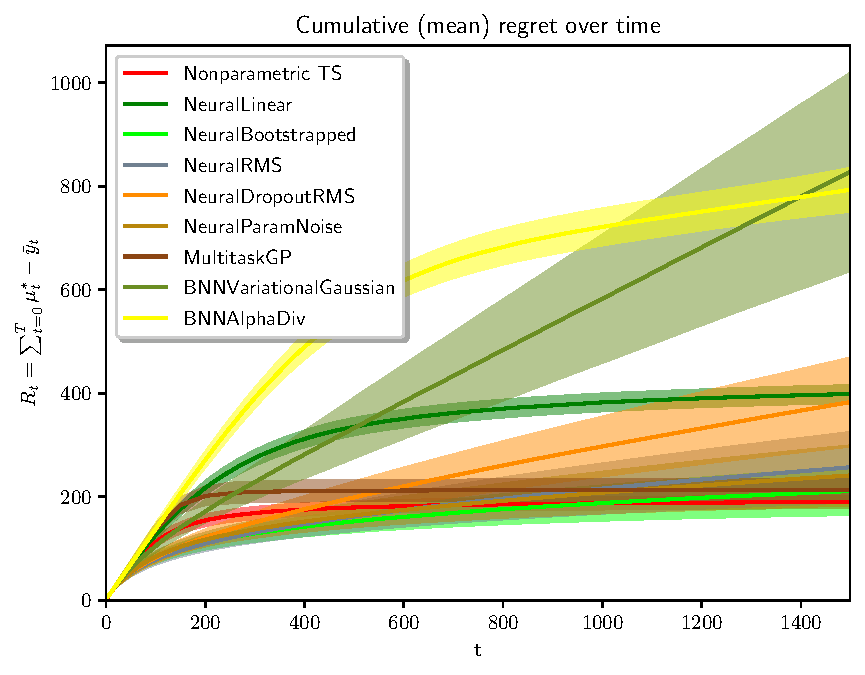
\includegraphics[width=\textwidth]{./figs/linear_showdown_baselines/cum_optexpected_regret_std}
		\vspace*{-5ex}
		\caption{Contextual linear Gaussian MAB, for $R=500$ realizations.}
		\label{fig:linear_showdown_baselines}
	\end{subfigure}
	\qquad
	\begin{subfigure}[c]{0.45\textwidth}
		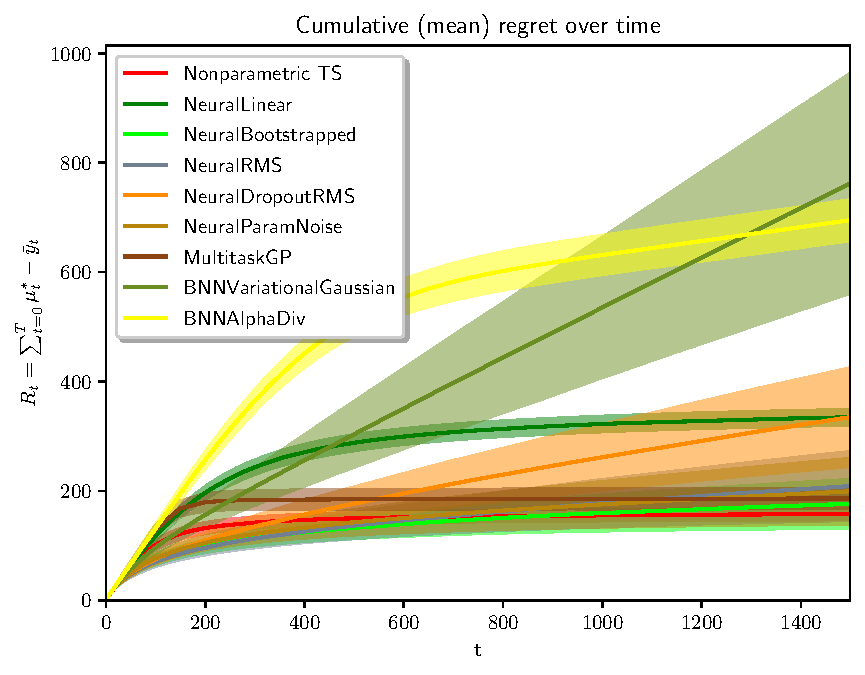
\includegraphics[width=\textwidth]{./figs/sparse_linear_showdown_baselines/cum_optexpected_regret_std}
		\vspace*{-5ex}
		\caption{Contextual sparse linear Gaussian MAB, for $R=500$ realizations.}
		\label{fig:sparse_linear_showdown_baselines}
	\end{subfigure}
	\vspace*{-2ex}
	\caption{Mean regret (standard deviation shown as shaded region) for 1000 independent realizations of the presented methods in all scenarios.}
	\label{fig:linear_gaussian_mixtures_baselines}
\end{figure}

